% Options for packages loaded elsewhere
\PassOptionsToPackage{unicode}{hyperref}
\PassOptionsToPackage{hyphens}{url}
%
\documentclass[
]{article}
\usepackage{amsmath,amssymb}
\usepackage{lmodern}
\usepackage{iftex}
\usepackage{graphicx}
\ifPDFTeX
  \usepackage[T1]{fontenc}
  \usepackage[utf8]{inputenc}
  \usepackage{textcomp} % provide euro and other symbols
\else % if luatex or xetex
  \usepackage{unicode-math}
  \defaultfontfeatures{Scale=MatchLowercase}
  \defaultfontfeatures[\rmfamily]{Ligatures=TeX,Scale=1}
\fi
% Use upquote if available, for straight quotes in verbatim environments
\IfFileExists{upquote.sty}{\usepackage{upquote}}{}
\IfFileExists{microtype.sty}{% use microtype if available
  \usepackage[]{microtype}
  \UseMicrotypeSet[protrusion]{basicmath} % disable protrusion for tt fonts
}{}
\makeatletter
\@ifundefined{KOMAClassName}{% if non-KOMA class
  \IfFileExists{parskip.sty}{%
    \usepackage{parskip}
  }{% else
    \setlength{\parindent}{0pt}
    \setlength{\parskip}{6pt plus 2pt minus 1pt}}
}{% if KOMA class
  \KOMAoptions{parskip=half}}
\makeatother
\usepackage{xcolor}
\usepackage{graphicx}
\makeatletter
\def\maxwidth{\ifdim\Gin@nat@width>\linewidth\linewidth\else\Gin@nat@width\fi}
\def\maxheight{\ifdim\Gin@nat@height>\textheight\textheight\else\Gin@nat@height\fi}
\makeatother
% Scale images if necessary, so that they will not overflow the page
% margins by default, and it is still possible to overwrite the defaults
% using explicit options in \includegraphics[width, height, ...]{}
\setkeys{Gin}{width=\maxwidth,height=\maxheight,keepaspectratio}
% Set default figure placement to htbp
\makeatletter
\def\fps@figure{htbp}
\makeatother
\setlength{\emergencystretch}{3em} % prevent overfull lines
\providecommand{\tightlist}{%
  \setlength{\itemsep}{0pt}\setlength{\parskip}{0pt}}
\ifLuaTeX
  \usepackage{selnolig}  % disable illegal ligatures
\fi
\IfFileExists{bookmark.sty}{\usepackage{bookmark}}{\usepackage{hyperref}}
\IfFileExists{xurl.sty}{\usepackage{xurl}}{} % add URL line breaks if available
\urlstyle{same} % disable monospaced font for URLs
\hypersetup{
  pdftitle={Progressive Hedging and Tabu Search Applied to Mixed Integer (0, 1) Multistage Stochastic Programming},
  hidelinks,
  pdfcreator={LaTeX via pandoc}}

\title{Progressive Hedging and Tabu Search Applied to Mixed Integer (0,
1) Multistage Stochastic Programming}
\author{Lorenzo Sciandra}
\date{2022}

\begin{document}
\maketitle

\emph{Authors: ARNE LOKKETANGEN, DAVID L. WOODRUFF}\\
\emph{Year: 1996}
\hypertarget{problema-in-questione}{%
\section{Problema in questione}\label{problema-in-questione}}
Molti problemi affrontati da chi deve compiere decisioni sono
caratterizzati da un \textbf{processo decisionale a più fasi} con
incertezza riguardo al futuro, recourse, ecc... Con \emph{multistage}
s'intende che devono essere compiute una sequenza di decisioni, mentre
con \emph{recourse} intendiamo che ad ogni punto decisionale è
disponibile nuova conoscenza (verificarsi di variabili randomiche).
Poichè queste fasi decisionali corrispondono ad istanti temporali sono
solitamente indicizzate da {\(t \in T = 1,...,\tau\)}. Sebbene sia
richiesto di prendere decisioni solamente riguardo al presente, con
l'uso degli indici sottolineiamo il fatto che prenderemo ulteriori
decisioni nel futuro e vogliamo "\emph{proteggerci}" (\emph{hedge})
dall'incertezza riguardo al futuro. Tutto questo ci permette di
incrementare il potere di modellazione e quindi la possibilità di
rappresentare modelli realistici, grazie alla \textbf{rappresentazione
degli eventi incerti attraverso l'uso di variabili randomiche}. A
livello teorico quest'ultime possono assumere moltissimi valori, ma non
si considerano funzioni di distribuzione di probabilità perchè non sono:
\begin{itemize}
\tightlist
\item
  \textbf{ragionevoli}: potrebbero non esserci abbastanza dati per
  stimare completamente distribuzioni multivariate;
\item
  \textbf{utili}: l'essenza stocastica può essere ben catturata da un
  numero ragionevole di \textbf{scenari rappresentativi}.
\end{itemize}
\hypertarget{scenari-rappresentativi}{%
\section{Scenari Rappresentativi}\label{scenari-rappresentativi}}
Ogni scenario {\(s \in \mathcal{S}\)} è specificato dando l'insieme
completo dell'assegnazione di valore alle variabili randomiche e da un
corrispondente valore di probabilità {\(Pr(s)\)}. Per ogni scenario
{\(s\)} e ogni istante decisionale {\(t\)} abbiamo un vettore di costi
{\(\mathbf{c}(s,t)\)} di dimensione {\(n(t)\)}, una matrice {\(A(s,t)\)}
di vincoli {\(m(t) \times n(t)\)} e un vettore {\(\mathbf{b}(s,t)\)} di
termini noti di lunghezza {\(m(t)\)}. Le variabili decisionali sono
rappresentate dal vettore {\(\mathbf{x}(s,t)\)} di dimensione {\(n(t)\)}
e dipendono strettamente dallo scenario. Viene indicato con
{\(\mathbf{X}\)} l'insieme di tutti i vettori per ogni istante temporale
e per ogni scenario, mentre con {\(\mathbf{X}(s)\)} l'insieme di tutti i
vettori {\(\mathbf{x}(s,t)\)} uno per istante temporale sullo scenario
fissato. Come si può notare il numero {\(n(t)\)} delle variabili che
compongono il vettore decisionale dello scenario dipende ovviamente
dall'istante temporale dato che istanti successivi possono avere nuove
realizzazioni. Questo vale anche per il numero di vincoli {\(m(t)\)}. Se
fossimo abbastanza preveggenti da sapere quale sarà la realizzazione
finale {\(s\)} e quindi anche i valori delle variabili casuali, il
nostro problema sarebbe:

\begin{equation*}
\begin{split} \min_{\mathbf{X}(s)} \:\:
f(s;\mathbf{X}(s)) \:\equiv & \: \sum_{t\in T} \sum_{i \in N(t)} c_i(s,t) \cdot x_i(s,t)\\
s.t \quad & \mathbf{A}(s)\cdot \mathbf{X}(s)\geq \mathbf{b}(s) \quad s \in \mathcal{S}\\
& x_i(s,t) \in \{0,1\}\quad i \in I(t), t \in T\\
& x_i(s,t) \geq 0 \quad i\in N(t)-I(t), t \in T
\end{split}
\end{equation*}

con {\(I(t)\)} l'insieme delle variabili intere ad ogni fase temporale.
Dato che non disponiamo dell'informazione su quale sarà lo scenario
{\(s\)} a realizzarsi dobbiamo leggermente modificare la funzione
obiettivo in modo da ottenere una soluzione che sia ammissibile
indipendentemente dallo scenario che capiterà. I sistemi di soluzione
{\(\mathbf{X}\)} che soddisfano i vincoli con probabilità 1 sono
chiamati \textbf{ammissibili}, ci riferiremo invece ad un vettore di
soluzioni del sistema come \textbf{implementabile} se per ogni coppia di
scenari {\(s,s^{\prime}\)} che risultano indistinguibili fino al tempo
{\(t\)} hanno {\(\mathbf{X}(s) = \mathbf{X}(s^{\prime})\)}. L'insieme
dei sistemi di soluzione che soddisfano tali proprietà viene indicato
con {\(\mathcal{N}_{\mathcal{S}}\)}, per un dato set di scenari
{\(\mathcal{S}\)}

\begin{equation*}
    \begin{split} \min_{\mathbf{X}}\:\:& \sum_{s\in S} Pr(s) \cdot f(s;\mathbf{X}(s)) = \sum_{s\in S} Pr(s) \cdot \sum_{t\in T} \sum_{i \in N(t)} c_i(s,t) \cdot x_i(s,t)\\
s.t \quad & \mathbf{A}(s)\cdot \mathbf{X}(s)\geq \mathbf{b}(s) \quad s \in \mathcal{S}\\
& x_i(s,t) \in \{0,1\}\quad i \in I(t), t \in T\\
& x_i(s,t) \geq 0 \quad i\in N(t)-I(t), t \in T\\
&\mathbf{X} \in \mathcal{N}_{\mathcal{S}}
\end{split}
\end{equation*}

Soluzioni non implementabili saranno scartate, mentre quelle non
ammissibili possono invece avere del valore utile. In generale
l'algoritmo di \textbf{progressive hedging} assicura soluzioni
implementabili ad ogni iterazione e ammissibili alla convergenza. L'approccio risolutivo proposto si applica in tutti contesti con
qualsiasi numero di variabili intere in ogni istante temporale e dove
ogni dato può potenzialmente essere stocastico. Dato che il metodo può
trattare istanze con numero variabile di istanti temporali, bisogna
abbandonare l'idea di trovare un metodo esatto e far uso di euristiche.

\hypertarget{metodo-risolutivo}{%
\section{Metodo Risolutivo}\label{metodo-risolutivo}}

\hypertarget{progressive-hedging}{%
\subsection{Progressive Hedging}\label{progressive-hedging}}

L'algoritmo di Progressive Hedging proposto da Rockafellar e Wets ha
buone proprietà teoriche: converge ad un ottimo globale nel caso
convesso e ha un tasso di convergenza lineare nel caso di problema
stocastico lineare e se converge nel caso non convesso allora converge
ad un ottimo locale. Per applicare il PH al nostro problema organizziamo
gli scenari e i tempi decisionali in un albero in cui ogni nodo foglia
rappresenta la realizzazione di uno scenario e ogni livello un istante
temporale diverso in cui le variabili randomiche assumeranno un certo
valore. Abbiamo quindi che ogni ramo dell'albero è uno scenario diverso e la radice rappresenta l'istante attuale. In questo modo due
realizzazioni diverse, ma che coincidono per parte del loro percorso
condivideranno dei nodi interni all'albero e di conseguenza gli stessi
valori delle variabili fino alla loro separazione, in questo modo
possiamo facilmente ottenere l'ammissibilità di cui parlavamo prima,
verificando che assumano esattamente i valori riportati nei nodi. Un
esempio di albero con {\(\tau = 3\)} e due decisioni per istante
temporale è:
\begin{figure}[h!]
    \centering
    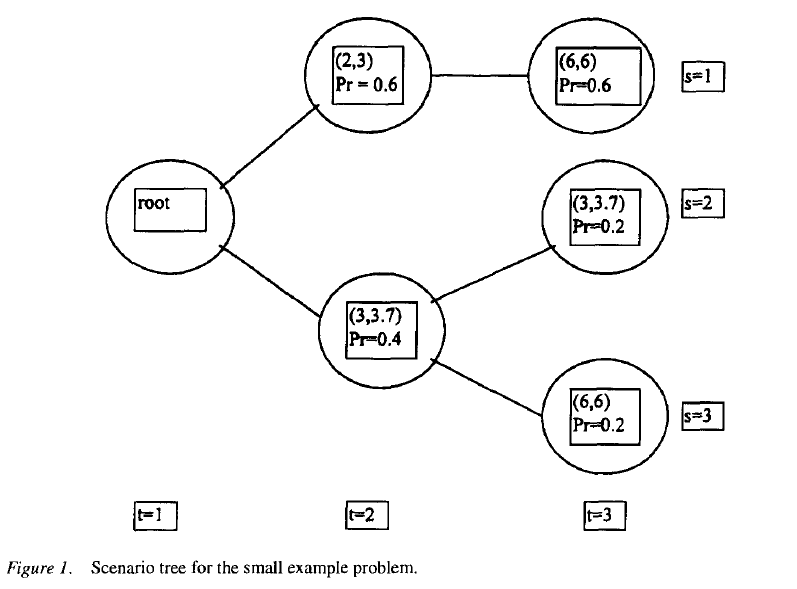
\includegraphics[width=0.8\columnwidth]{Images/ScenarioTree.png}
    %\caption{Caption}
    \label{fig:ScenatioTree}
\end{figure}


La funzione obiettivo del nostro problema cerca quindi il ramo
nell'albero che minimizza il costo rispettando i vincoli ad ogni nodo e
in modo che sia implementabile. L'idea è quella di ottenere per ogni
scenario {\(s\)} una soluzione approssimata che tenga in conto i
vincoli, la funzione obiettivo deterministica {\(f_{s}\)} più una
penalità in caso di mancata implementabilità. L'algoritmo ha il seguente pseudocodice:

\begin{figure}[h!]
    \centering
    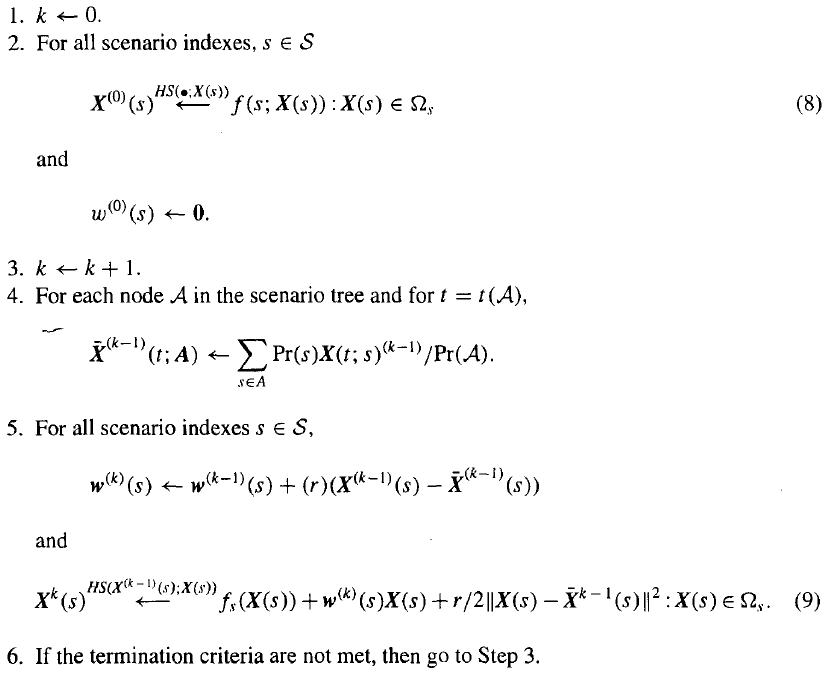
\includegraphics[width=1\columnwidth]{Images/ProgressiveHedgingandTabuSearch.png}
    %\caption{Caption}
    \label{fig:ProgressiveHedgingandTabuSearch}
\end{figure}

Considerazioni sullo pseudocodice:
\begin{itemize}
\tightlist
\item
  {\(Pr(\mathcal{A})\)} è la somma di tutte le probabilità {\(Pr(s)\)}
  di tutti gli scenari che si dipartano dal nodo {\(\mathcal{A}\)};
\item
  {\(t(\mathcal{A})\)} è l'istante temporale (livello) a cui si trova il
  nodo {\(\mathcal{A}\)} nell'albero;
\item
  l'assegnamento {\((8)\)} significa \emph{"assegna il risultato di una
  ricerca d'ottimizzazione euristica {\(HS\)} che cerca di trovare il
  migliore argomento {\(\mathbf{X}(s)\)} che minimizza la parte destra
  dell'espressione"};
\item
  l'espressione {\(\mathbf{X}(t;\mathcal{A})\)} viene usata per indicare
  l'assegnamento dei vettori decisionali per ogni scenario che passa per
  il nodo {\(\mathcal{A}\)} fino al tempo {\(t\)};
\item
  l'apice nei vettori/variabili serve per tenere in considerazione
  l'iterazione;
\item
  il primo e il terzo for ({\(1.\)} e {\(5.\)}) ciclano sulle foglie o
  realizzazioni degli scenari, mentre il secondo su tutti i nodi
  dell'albero. In particolare {\(\mathbf{X}(s)\)} è la soluzione
  euristica calcolata per uno scenario, mentre
  {\(\overline{\mathbf{X}}(t;\mathcal{A})\)} è una stima delle soluzioni
  originate da un nodo interno come sommatoria pesata delle foglie che
  origina per la loro probabilità di verificarsi;
\item
  i vettori {\(\mathbf{w}(s)\)} possono essere intesi come variabili
  duali, come prezzi ombra per l'implementabilità dei vincoli;
\item
  le condizioni di terminazione sono basate sia sulla convergenza e
  quindi le iterazioni continuano fino a quando
  {\({\overline{\mathbf{X}}}^{k}(s)\)} è prossimo a
  {\({\overline{\mathbf{X}}}^{k - 1}(s)\)} per ogni scenario {\(s\)},
  misura ad esempio con classica distanza euclidea. Bisogna anche tenere
  traccia del tempo/numero di iterazione massimo perchè è possibile
  anche la non convergenza.
\end{itemize}

\hypertarget{ricerca-euristica}{%
\subsection{Ricerca Euristica}\label{ricerca-euristica}}

Lo pseudocodice mostrato prima necessità di risolvere due problemi di
ricerca, quelli etichettati con {\((8)\)} e {\((9)\)}. Il primo è un
problema di programmazione lineare mista, mentre il secondo è simile ma ha termini quadratici nella funzione obiettivo. I due problemi si
differenziano per la soluzione iniziale di partenza per poi usare
un'euristica basata sulla Tabu Search proposta da Glover:

\begin{enumerate}
\tightlist
\item
  Considera le mosse di pivot che portano a soluzioni adiacenti che
  siano ammissibili per il problema rilassato (rilassamento continuo per
  problema di programmazione lineare mista). Se una mossa candidata ci
  conduce ad una soluzione ammissibile intera {\(x\)} il cui valore di
  funzione obiettivo {\(z < z^{\ast}\)} è migliore del migliore valore
  trovato finora, diventa la nuova migliore soluzione {\(x^{\ast}\)};
\item
  Seleziona tra le precedenti mosse quella con la valutazione più alta
  ottenuta applicando la tabu restrictions e l'aspiration criteria;
\item
  Esegui la mossa selezionata aggiornando la memoria della tabu search e
  le altre strutture dati usate per guidare la ricerca. A meno che si
  incontri il criterio di stop ripeti dal passo 1.
\item
  (solo per il passo {\((9)\)}) Fissa i valori interi affinchè
  corrispondano con quelli trovati nella miglior soluzione durante la
  ricerca e risolvi il rilassamento continuo per fissare invece i valori
  continui.
\end{enumerate}
La soluzione di partenza per {\((8)\)} è ottenuta risolvendo il suo
rilassamento continuo usando MINOS (Murtagh and Saunders, 1993), per
{\((9)\)} si usa la soluzione {\(\mathbf{X}^{(k - 1)}(s)\)} per fissare
i valori delle variabili intere e dopo si usa sempre MINOS per ottenere
la soluzione di partenza.
\hypertarget{uso-della-tabu-search}{%
\subsubsection{Uso della Tabu Search}\label{uso-della-tabu-search}}
Precisiamo il modo in cui viene usata la Tabu Search al passo {\(2.\)}
Le mosse vengono tra loro distinte in base all'indice della variabile
che fanno uscire dalla base. Dopo che una variabile ha lasciato la base
non vi entrerà almeno per un numero stabilito di iterazioni che viene
scelto in maniera randomica nell'intervallo {\((n/15,n/7)\)} dove
{\(n\)} è il numero di variabili totali. La valutazione di una mossa
tiene in conto sia il valore della funzione obiettivo sia una misura
dell'ammissibilità intera, in particolare per passare dalla soluzione
{\(i\)} alla {\(j\)} si prende in considerazione
{\(\Delta z(j) = z(i) - z(j)\)} per il cambiamento nella funzione
obiettivo e {\(\Delta u(j) = u(i) - u(j)\)} dove {\(u\)} è la somma
delle differenze tra il valore di ogni variabile intera e l'intero a
loro più vicino (\emph{total integer infeasibility}). A seconda dei
valori di {\(z(j)\)} e {\(u(j)\)} le mosse vengono assegnate a
\textbf{tipi} diversi con associata una diversa \textbf{funzione di
rank}. Le mosse vengono ordinate prima rispetto al tipo e poi, mosse
dello stesso tipo, vengono ordinate in base al valore decrescente della
funzione di rank. La mossa da eseguire viene selezionata in modo
probabilistico ripetendo i seguenti passi:
\begin{enumerate}
\tightlist
\item
  prendi la mossa in cima alla lista per priorità;
\item
  accettala se sarebbe la migliore vista;
\item
  rifiutala se è tabu e piazzala in fondo alla lista, togliendole lo
  status di tabu per l'iterazione corrente;
\item
  se la mossa è degenere rifiutala e rimuovila dalla lista;
\item
  genera un numero pseudocasuale {\(r\)} campionato da una distribuzione
  uniforme {\((0,1)\)}. Se {\(r > p\)} rifiutalo e rimuovilo dalla lista
  e ritorna al passo 1, altrimenti accetta la mossa, dove {\(p\)} è un
  parametro che va definito.
\end{enumerate}

\hypertarget{conclusioni}{%
\section{Conclusioni}\label{conclusioni}}

L'articolo introduce la prima implementazione di un metodo
general-purpose per trovare buone soluzioni ad un problema di
programmazione mista stocastico e multistage. Questo viene fatto usando
la tabu search per i sottoproblemi ed un progressive hedging per
coordinare la fusione tra le soluzioni dei sottoproblemi con le nozioni
della convergenza intera. Forse i miglioramenti più sorprendenti possono
essere ottenuti raggruppando più scenari, risolvendo il minor numero
risultante di sottoproblemi più grandi e combinando queste soluzioni.
Una ricerca potrebbe essere fatta per comprendere se sia meglio
partizionare gli scenari per ottenere facili soluzioni dai sottoproblemi
risultati o per accelerare la convergenza. Sono anche possibili
miglioramenti per la ricerca di soluzioni a problemi quadratici 0-1,
nello specifico ci sarebbe bisogno per criterio di stop adattivo che
possa essere usato dalla tabu search per ottenere buone soluzioni.
Questo comporterebbe l'eliminazione o il rimpiazzamento di parametri di
controllo.

\end{document}